\section{Motivation}
\label{sec:motivation}

Historically, using the alignment and motion of human limbs as an input modality for human-computer interfaces has been accomplished through intrusive methods --- by placing markers or sensors on the body. Up until recently, non-intrusive sensing of human limb positions has been limited to research efforts (see \textcite{Moeslund:2006}; \textcite{Porta:2002}; \textcite{Moeslund:2001}; and \textcite{Gavrila:1999} for surveys of these works). In recent years, vision-based skeletal tracking sensors have become commercially available from a variety of established vendors such as Microsoft\footnote{\href{http://www.microsoft.com/en-us/kinectforwindows/}{microsoft.com/en-us/kinectforwindows}} (Figure~\ref{fig:kinect}) and Asus\footnote{\href{http://www.asus.com/Multimedia/Motion_Sensor_Products/}{www.asus.com/Multimedia/Motion\_Sensor\_Products}}. Non-intrusive --- or \emph{perceptual} \parencite{Turk:2000, Crowley:2000} --- sensing of body movements has thus become widely accessible for both commercial and non-commercial applications \parencite{Francese:2012}.

\begin{SCfigure}[3][ht]
\centering
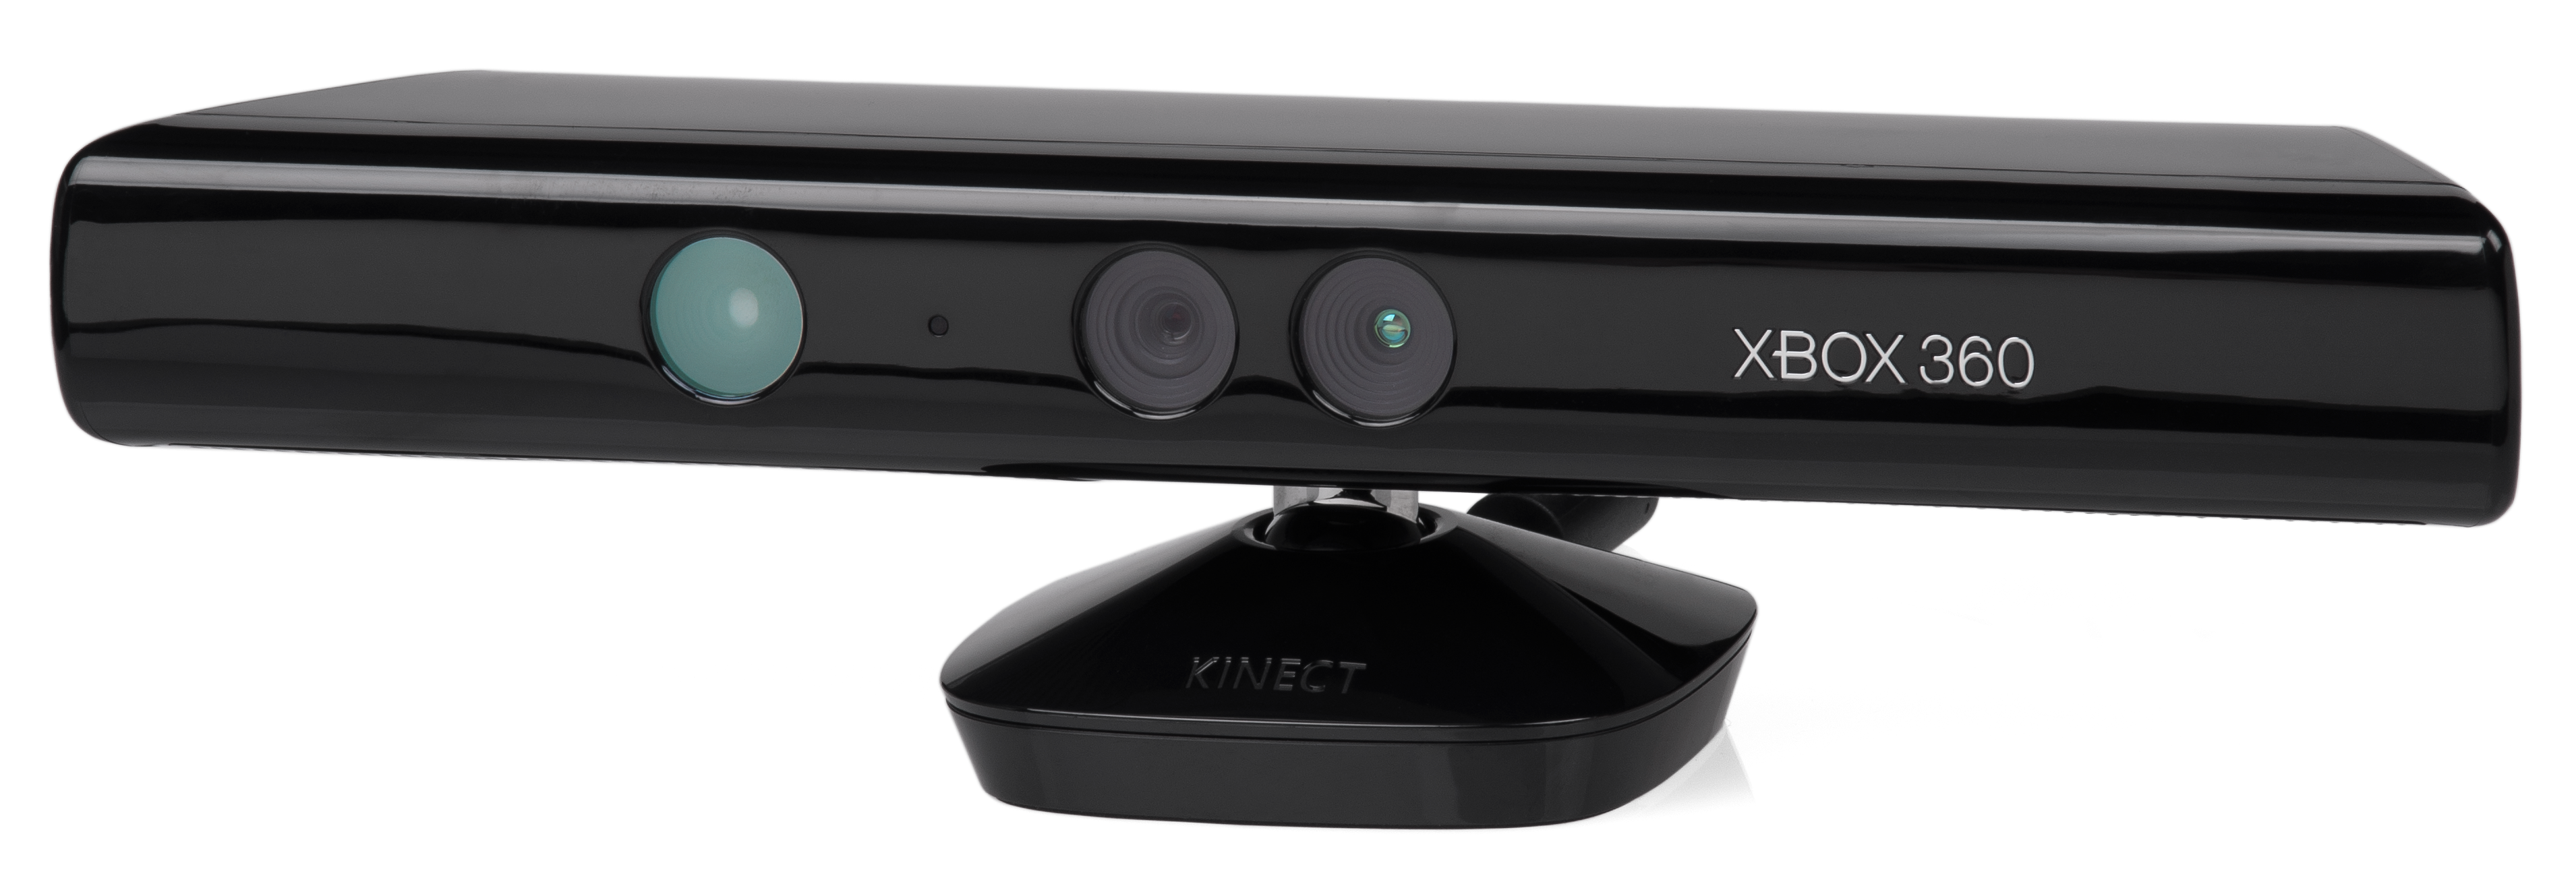
\includegraphics[width=.4\textwidth]{kinect}
\caption{The Microsoft Kinect sensor is equipped with a depth camera that can "see" the positions and motion of human limbs.}
\label{fig:kinect}
\end{SCfigure}

There are a variety of computing applications where the non-intrusive detection of human limb positions can be desirable as an input modality. Gaming is an obvious one (see Figure~\ref{fig:kinect-gaming}), where using movements with "prior mappings" to real-world happenings increases immersion \parencite{Cairns:2014}. Another one is user interfaces on public interactive systems: An input modality that does not require physical contact is often cheaper to deploy and maintain, and more hygienic to use. Of course, there are numerous other contexts where hygiene considerations can make a touch-less interface desirable: Cooking, gardening, working on a dirty mechanism, and performing surgery \parencite{Wen:2013} come to mind. Other applications for perceptual interfaces include convenient control of smart homes \parencite{Tang:2013}, interactive art and musical instruments\footnote{\href{http://vimeo.com/45417241}{vimeo.com/45417241}}, interfaces for manipulating 3D images \parencite{Gallo:2013}, and spatial medicine \parencite{Lozano-Quilis:2013, Huang:2011, Simmons:2013}.

\begin{SCfigure}[\sidecaptionrelwidth][ht]
\centering
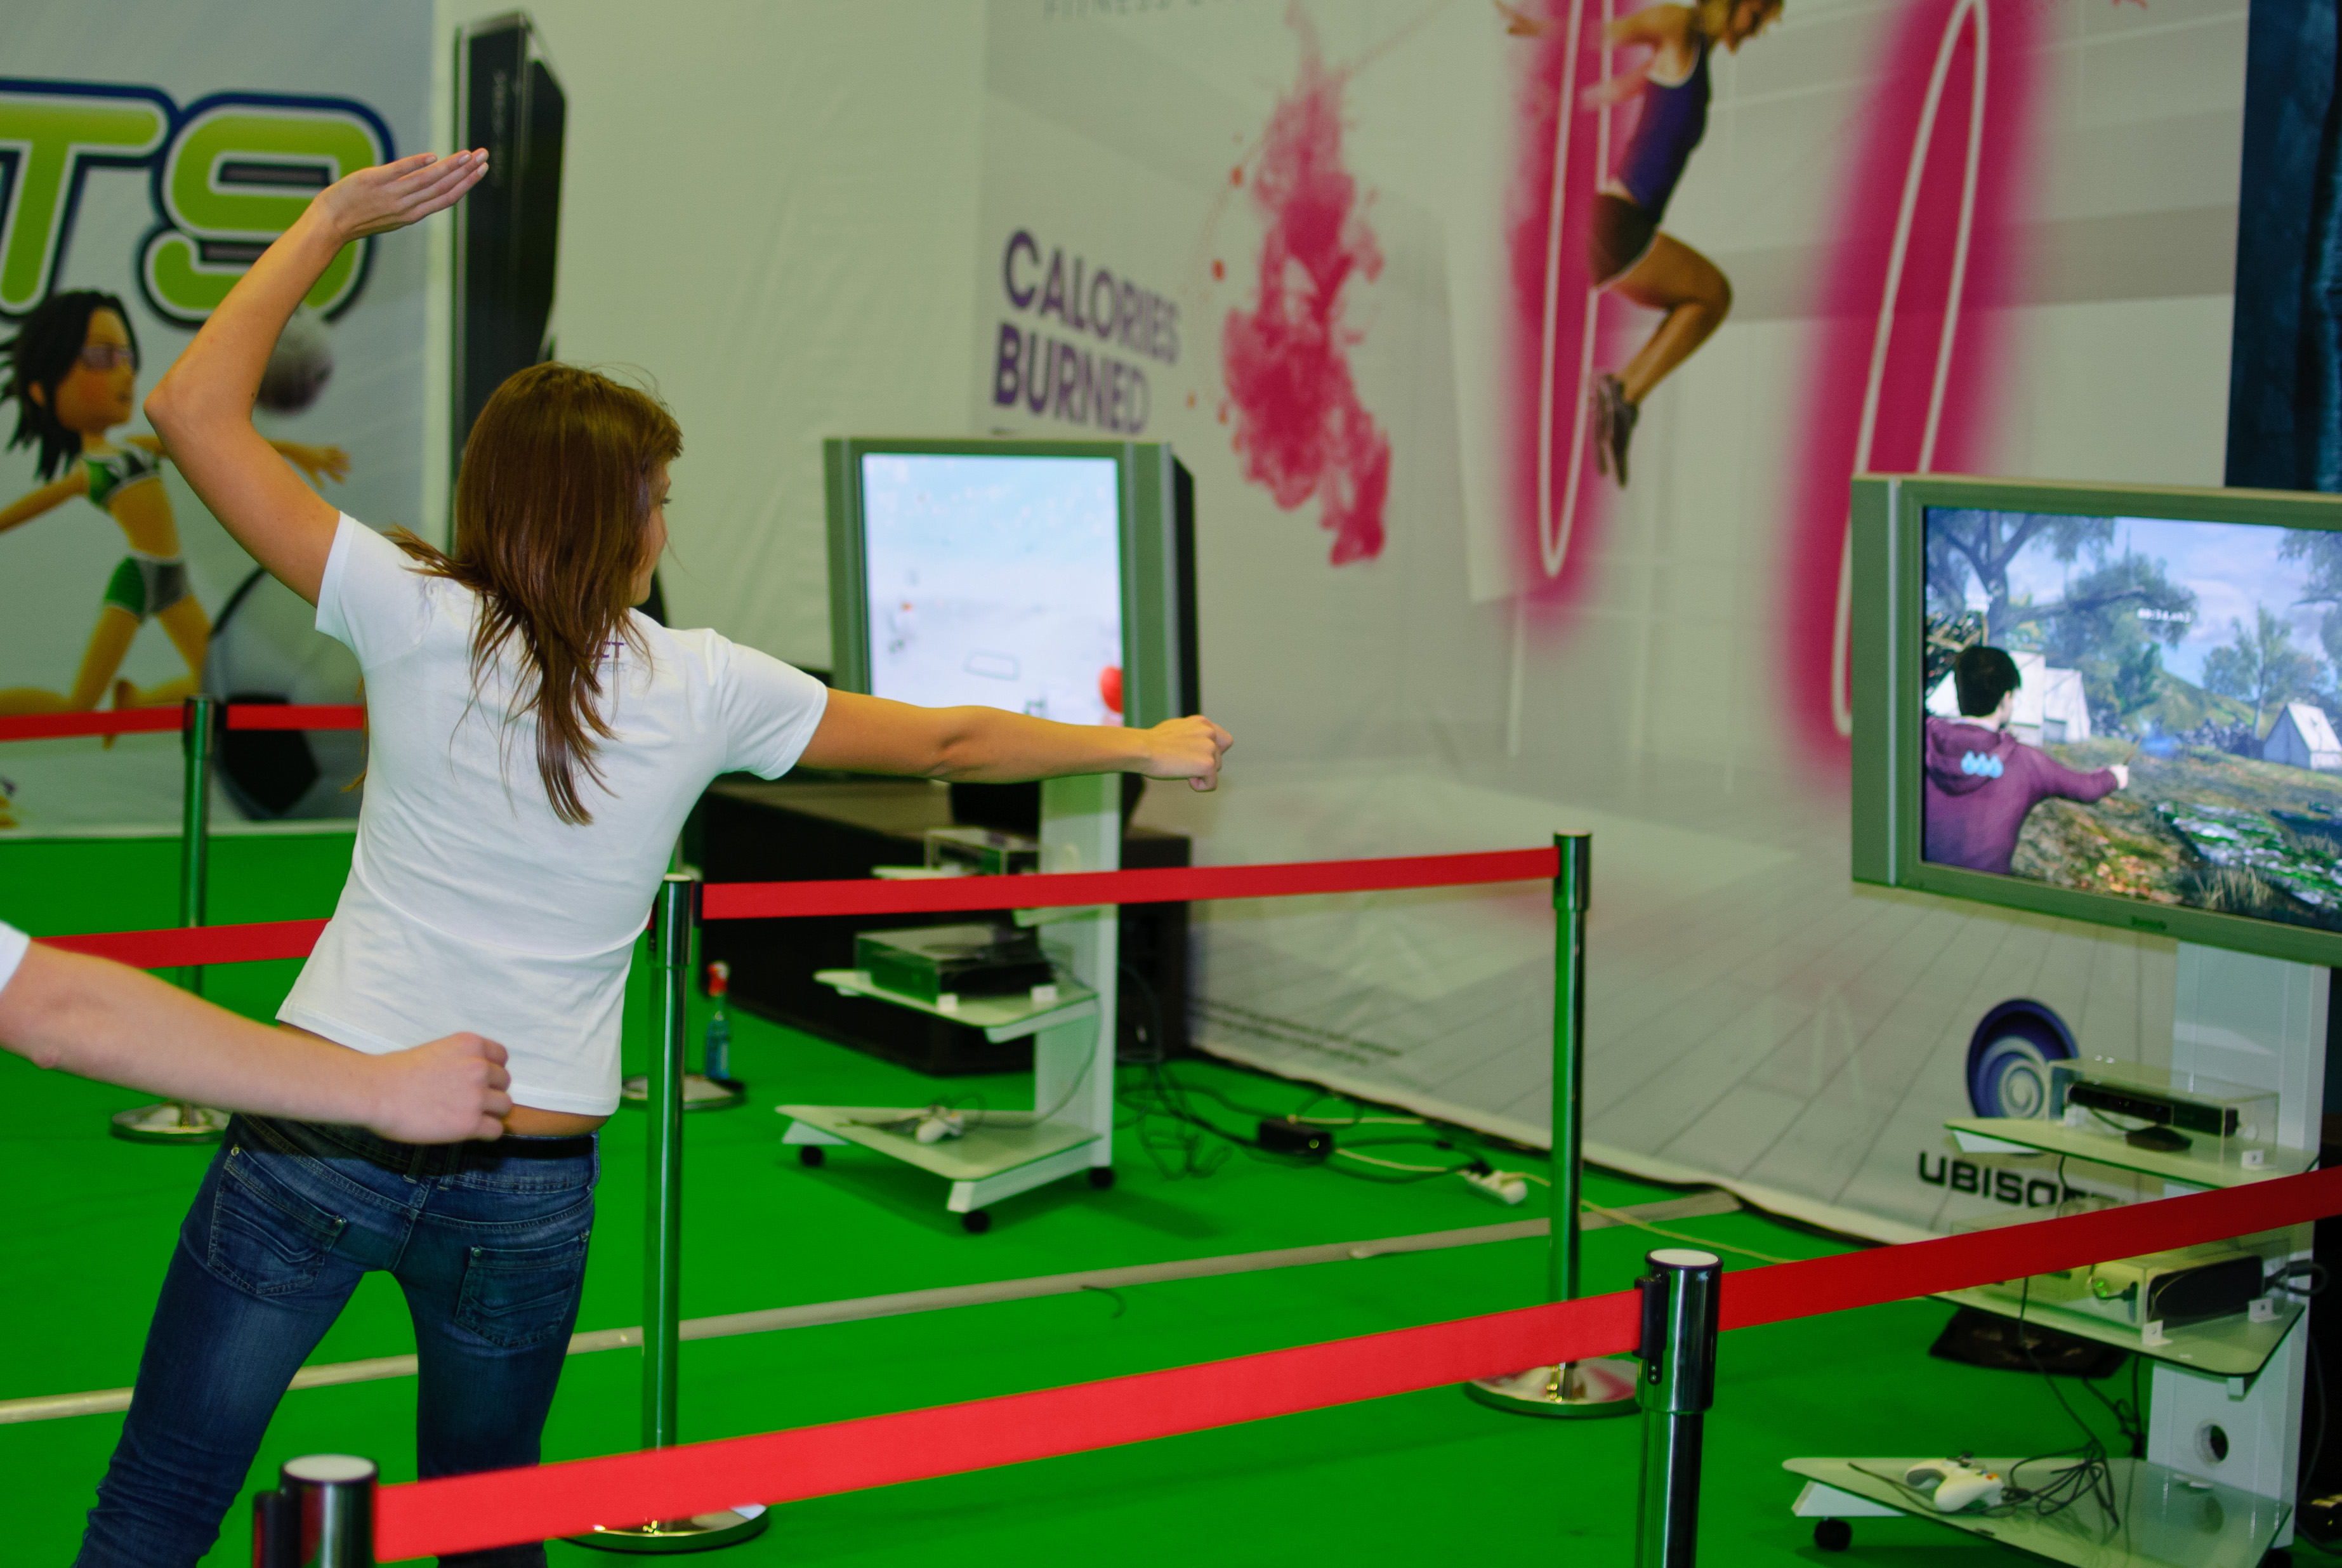
\includegraphics[width=.5\textwidth]{kinect-gaming}
\caption{Gaming with the Microsoft Kinect. The sensor detects the motion of large human limbs without requiring any markers or devices to be worn or wielded.}
\label{fig:kinect-gaming}
\end{SCfigure}

The design and development of perceptual interfaces requires that \emph{gestures} --- limb positions and movements that constitute inputs to the interface --- be programmed \parencite{Lu:2012} --- or \emph{authored} \parencite{Kim:2013, Hartmann:2007} --- in a machine-readable manner and mapped to events within the interactive system. This can be done in a textual programming environment using tools supplied by vendors of gesture-sensing hardware\footnote{\href{http://www.microsoft.com/en-us/kinectforwindowsdev/}{microsoft.com/en-us/kinectforwindowsdev}}\footnote{\href{http://www.softkinetic.com}{softkinetic.com}} or third parties\footnote{\href{http://kinecttoolbox.codeplex.com}{kinecttoolbox.codeplex.com}}. Using textual programming to author gestures, however, has drawbacks --- both for adept software developers and for comparatively non-technical users such as designers, artists, hobbyists or researchers in fields other than computing. (Borrowing the definition from \textcite{Ko:2011}; I will henceforth refer to these users who use or produce software not as an end, but as a means towards goals in their own domain, as \emph{end-users}). These drawbacks can be expressed in terms of \posscite{Norman:1986, Norman:2002} concepts of the \emph{gulf of execution} and the \emph{gulf of evaluation}. Specifically; for end-users, textual programming embodies a significant \emph{gulf of execution} --- a chasm between the user's goals and the actions taken within a system to achieve those goals – since it introduces additional tasks like setting up the programming environment and getting used to the development ecosystem. For both end-users and software developers, textual programming embodies a significant \emph{gulf of evaluation} --- a gap between a system's output and the users's expectations and intentions --- since itt does not allow for rapid testing of whether an authored gesture specification conforms to the design that the user has in mind. (See Figure~\ref{fig:gulfs} for a visualization of the \emph{gulf of execution} and the \emph{gulf of evaluation}.) From a software engineering perspective, \textcite{Hoste:2014} suggest that imperative textual programming “cannot cope” with mid-air gestures “due to the inversion of control where the execution flow is defined by input events rather than by the program, the high programming effort for maintaining an event history and the difficulty of expressing complex patterns.” Thus, textual programming does not fully support the embodied \parencite{Dourish:2004},  reflective \parencite{Schon:1984}, and experiential \parencite{Lindell:2014} practices inherent in the design, construction and evaluation \parencite{Hartmann:2006} of these highly interactive artifacts \parencite{Myers:2000, Lim:2008}.

\begin{SCfigure}[\sidecaptionrelwidth][ht]
\centering
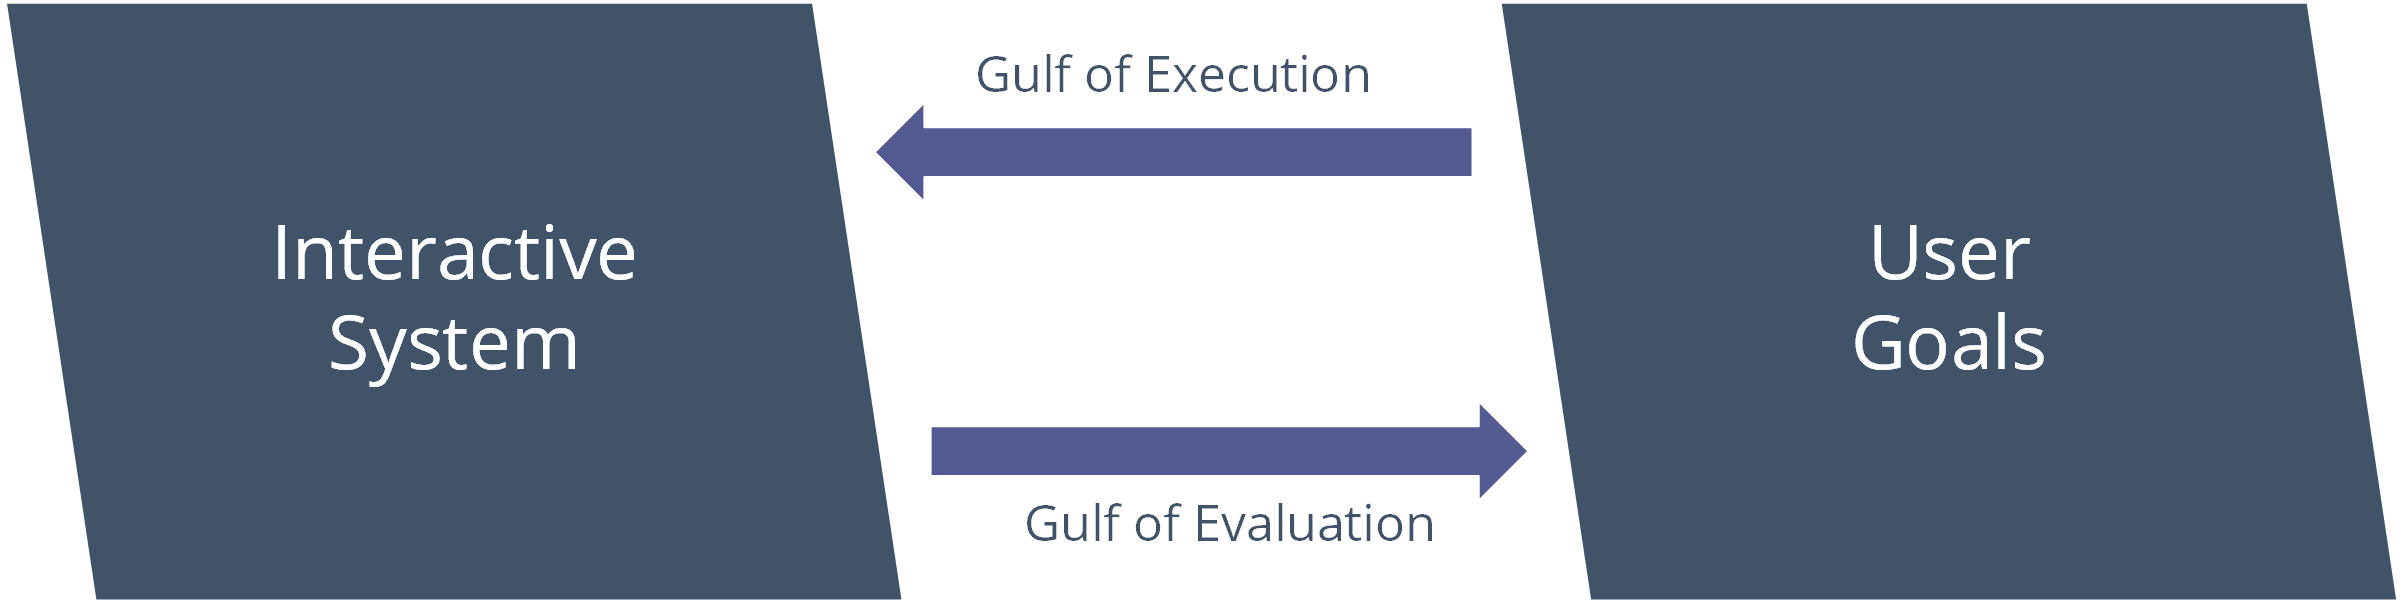
\includegraphics[width=0.7\textwidth]{gulfs}
\caption{The \emph{gulf of execution} and the \emph{gulf of evaluation}. The gulfs pertain to unidirectional aspects of interaction: The \emph{gulf of execution} lies between the user's goals and the interactive system; the \emph{gulf of evaluation} divorces the interactive system from the users's expectations and intentions.}
\label{fig:gulfs}
\end{SCfigure}

Using appropriate user interfaces for a job helps bridge the gulfs of evaluation and execution \parencite{Norman:2002}.

This thesis presents my attempt at producing an appropriate \hl{user interface to support the design and development of perceptual gesture-based interfaces by end-users.}

\section{Aim} %-----------------------------------------------------------------

The \hl{aim} of this thesis is to \hl{document the design, development, deployment and evaluation of a \emph{software application to support end-users' authoring gross mid-air gestures} for \emph{skeletal tracking perceptual input devices}}.

The term \hl{\emph{end-user} refers to those who utilize or produce software as a means towards goals in their own domain}, rather than producing computing applications as an end \parencite{Ko:2011}.\ A mid-air gesture authoring tool may target diverse populations of end users including designers, artists, hobbyists, gamers and educators.

The methods employed in the design and evaluation of the application are selected to be appropriate for these purposes. The practices employed for the construction and deployment of the application also reflect its end-user focus: The application must perform well and reliably on users' computers, be easy to obtain and set up, and be maintainable to facilitate rapid adaptation to evolving technologies and user needs \parencite{McConnell:2009, Brooks:1995}.

\subsection{Research Questions} %-----------------------------------------------

The main research question pursued in this thesis is as follows:

\begin{itemize}
\item \hl{\emph{How can end-users' authoring of gross mid-air gestures for skeletal tracking interfaces be supported with a software tool?}}
\end{itemize}

The main research question engenders the following secondary questions that align with the research:

\begin{itemize}
\item What are the \hl{desiderata and design considerations} that would pertain to mid-air gesture authoring software for end-users?
\item What methods are appropriate to \hl{evaluate} the application?
\end{itemize}

\subsection{Hypothesis and Expected Contributions}

I hypothesize that a suitably designed gesture authoring tool will accomplish the following:

\begin{itemize}
\item It will \hl{enable \emph{end-users} with no experience in textual programming and/or gestural interfaces to introduce gesture control} to computing applications that serve their own goals.
\item It will \hl{provide \emph{developers} and \emph{designers} of gestural interfaces with a rapid prototyping tool} that can be used to experientially evaluate designs.
\end{itemize}

I expect the following to be the \emph{contributions} of this work:

\begin{enumerate}
\item \emph{A software application} for authoring mid-air gestures that will accomplish the goals above and constitue an authentic contribution as an artifact of research through design.
\item Insights derived from the design, development, deployment and evaluation of the gesture authoring software that may inform future interaction design research and practice.
\end{enumerate}

The software application constitutes an artifact of \hl{\emph{research through design}} \parencite{Frayling:1993}. Thus, it is expected to fullfill the following criteria proposed by \textcite{Zimmerman:2007} for the evaluation of such artifacts:

\begin{itemize}
\item \emph{Process.} The methods employed must be selected rationally and documented rigorously.
\item \emph{Invention.} Various topics must be integrated in a novel fashion to create the artifact.
\item \emph{Relevance.} The artifact must be situated within a real, current context; while supporting a shift towards a justifiably preferable state.
\item \emph{Extensibility.} The work must enable the future exploitation of the knowledge derived from it.
\end{itemize}

\section{Scope}
\label{sec:scope}

This section defines the scope of the research presented in this thesis. Table~\ref{tab:scope-summary} presents a summary of the scope, while the text serves to elaborate on details and clarify the terminology used.

In human-computer interaction (HCI) and interaction design (IxD) literature, the usage of the word \emph{gesture} is ambiguous: Depending on the context, it may denote finger strokes on a touchscreen \parencite{Lu:2013}, deformations inflicted on a tangible input device \parencite{Warren:2013}, full-body poses \parencite{Walter:2013}, even finger movements on a keyboard \parencite{Zhang:2014}. For the purporses of this thesis; the following definition, adapted from \textcite{Kurtenbach:1990}, will be used:

\begin{quote}
\emph{A gesture is a movement or position of a human body part that conveys information.}
\end{quote}

By design, in order to accomodate existing works, this definition is broad. It allows for the use of any body part in gesturing as well as the use of sensing devices such as mouse, styli and gloves. It does not require an explicit intention to justify gesturing, thus accommodating non-command user interfaces \parencite{Nielsen:1993} such as those that respond to affective \parencite{Kapur:2005} and habitual \parencite{Liu:2009} gestures.

More specifically, I use the term \hl{\emph{mid-air gestures}} to denote gestures that are performed in a volume where limbs can move freely in 3 dimensions; e.g. free space. This excludes gestures that are constrained to affect a tangible surface or a controller device that mechanically changes form; e.g. a keyboard, a touch-sensitive surface, or a shape display \parencite{Follmer:2013}.

The gesture sensing input device used during the course of this work was a Microsoft \emph{Kinect for Xbox 360}; chosen from among alternatives due to its availability. The device employs an infrared projector-camera pair to capture 3D \emph{depth images}. If what resembles a typical human body is present in the depth image, the positions (relative to the sensor) of its large limbs are detected using machine learning \parencite{Girshick:2011, Shotton:2011, Shotton:2012, Shotton:2013}. A \emph{skeletal model} of the user is produced in this fashion (Figure~\ref{fig:intro-skeleton}). The alignment and motion of the skeletal model is then used to to control interactive applications. This type of gesture-sensing hardware is said to detect the movements and/or location of human body parts \hl{\emph{perceptually}} --- without requiring physical contact \parencite{Turk:2000, Crowley:2000}. This excludes, from the scope of this thesis, systems that sense gestures using devices that must be worn, wielded, or touched --- e.g. a mouse, a stylus, a ring\footnote{\href{http://www.wearfin.com/}{wearfin.com}}\footnote{\href{https://www.hellonod.com/}{hellonod.com}}, or an accelerometer \parencite{Kela:2006, Ashbrook:2010}.

\begin{SCfigure}[\sidecaptionrelwidth][ht]
\centering
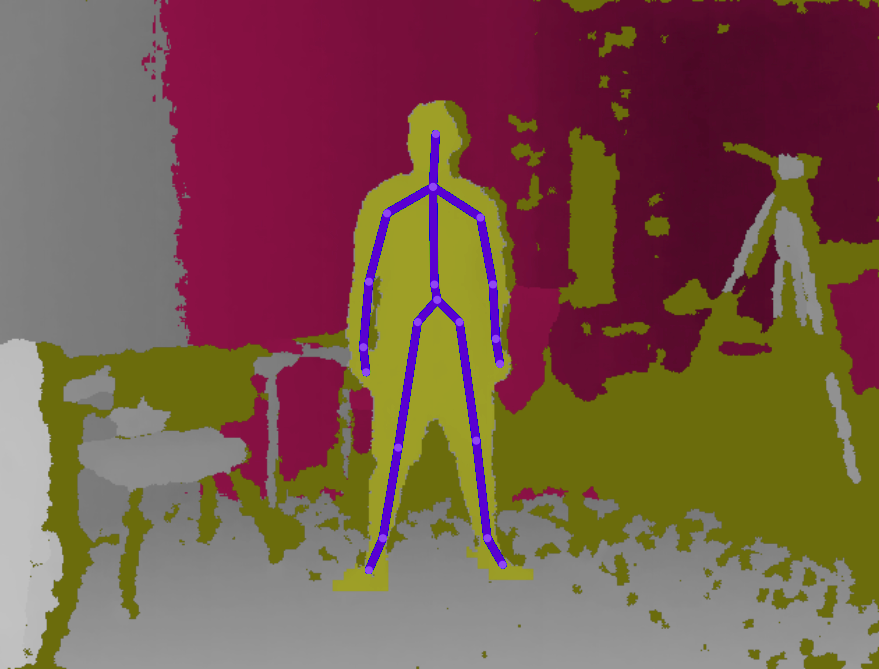
\includegraphics[width=0.5\textwidth]{intro-skeleton}
\caption{The Microsoft Kinect sensor employs an infrared projector-camera pair to capture 3D depth images, and fits a skeletal model onto what resembles a  human body in the image.}
\label{fig:intro-skeleton}
\end{SCfigure}

The Microsoft \emph{Kinect for Windows Software Development Kit (SDK)} version 1.8 was used to implement gesture sensing. The capabilities of the Kinect sensor and the SDK are not limited to skeletal tracking; they also include the detection of hand gestures, speech recognition, background removal from videos, facilitating proxemic interaction \parencite{Ballendat:2010}, fusing color and 3D images, and fusing data from multiple sensors. These topics, however, lie outside the scope of this work.

In kinesiology, human movements are classified according to movement precision \parencite{Haibach:2011}: \emph{Gross motor skills} denote large and comparatively imprecise movements produced by large muscles; e.g. jumping, or lifting weights. \emph{Fine motor skills} involve smaller movements with higher accuracy and precision; e.g. typing, or writing. Gestures do not always belong strictly to one of two discrete classes. Rather, the distinction between fine and gross gestures forms a continuum characterized by the size of the engaged musculature and the trade-off between force and precision \parencite{Edwards:2010} (Figure~\ref{fig:fine-gross-continuum}). One limitation of the skeletal tracking technology used for this work is that it can only detect gross gestures\footnote{Currently, the Kinect SDK does have support for hand gestures. However, this feature was not available while the design work described in this thesis was done.}. Thus, this work deals specifically with issues related to the use of \hl{\emph{gross movements}} of the human limbs as an interaction modality in computing.

\begin{SCfigure}[\sidecaptionrelwidth][ht]
\centering
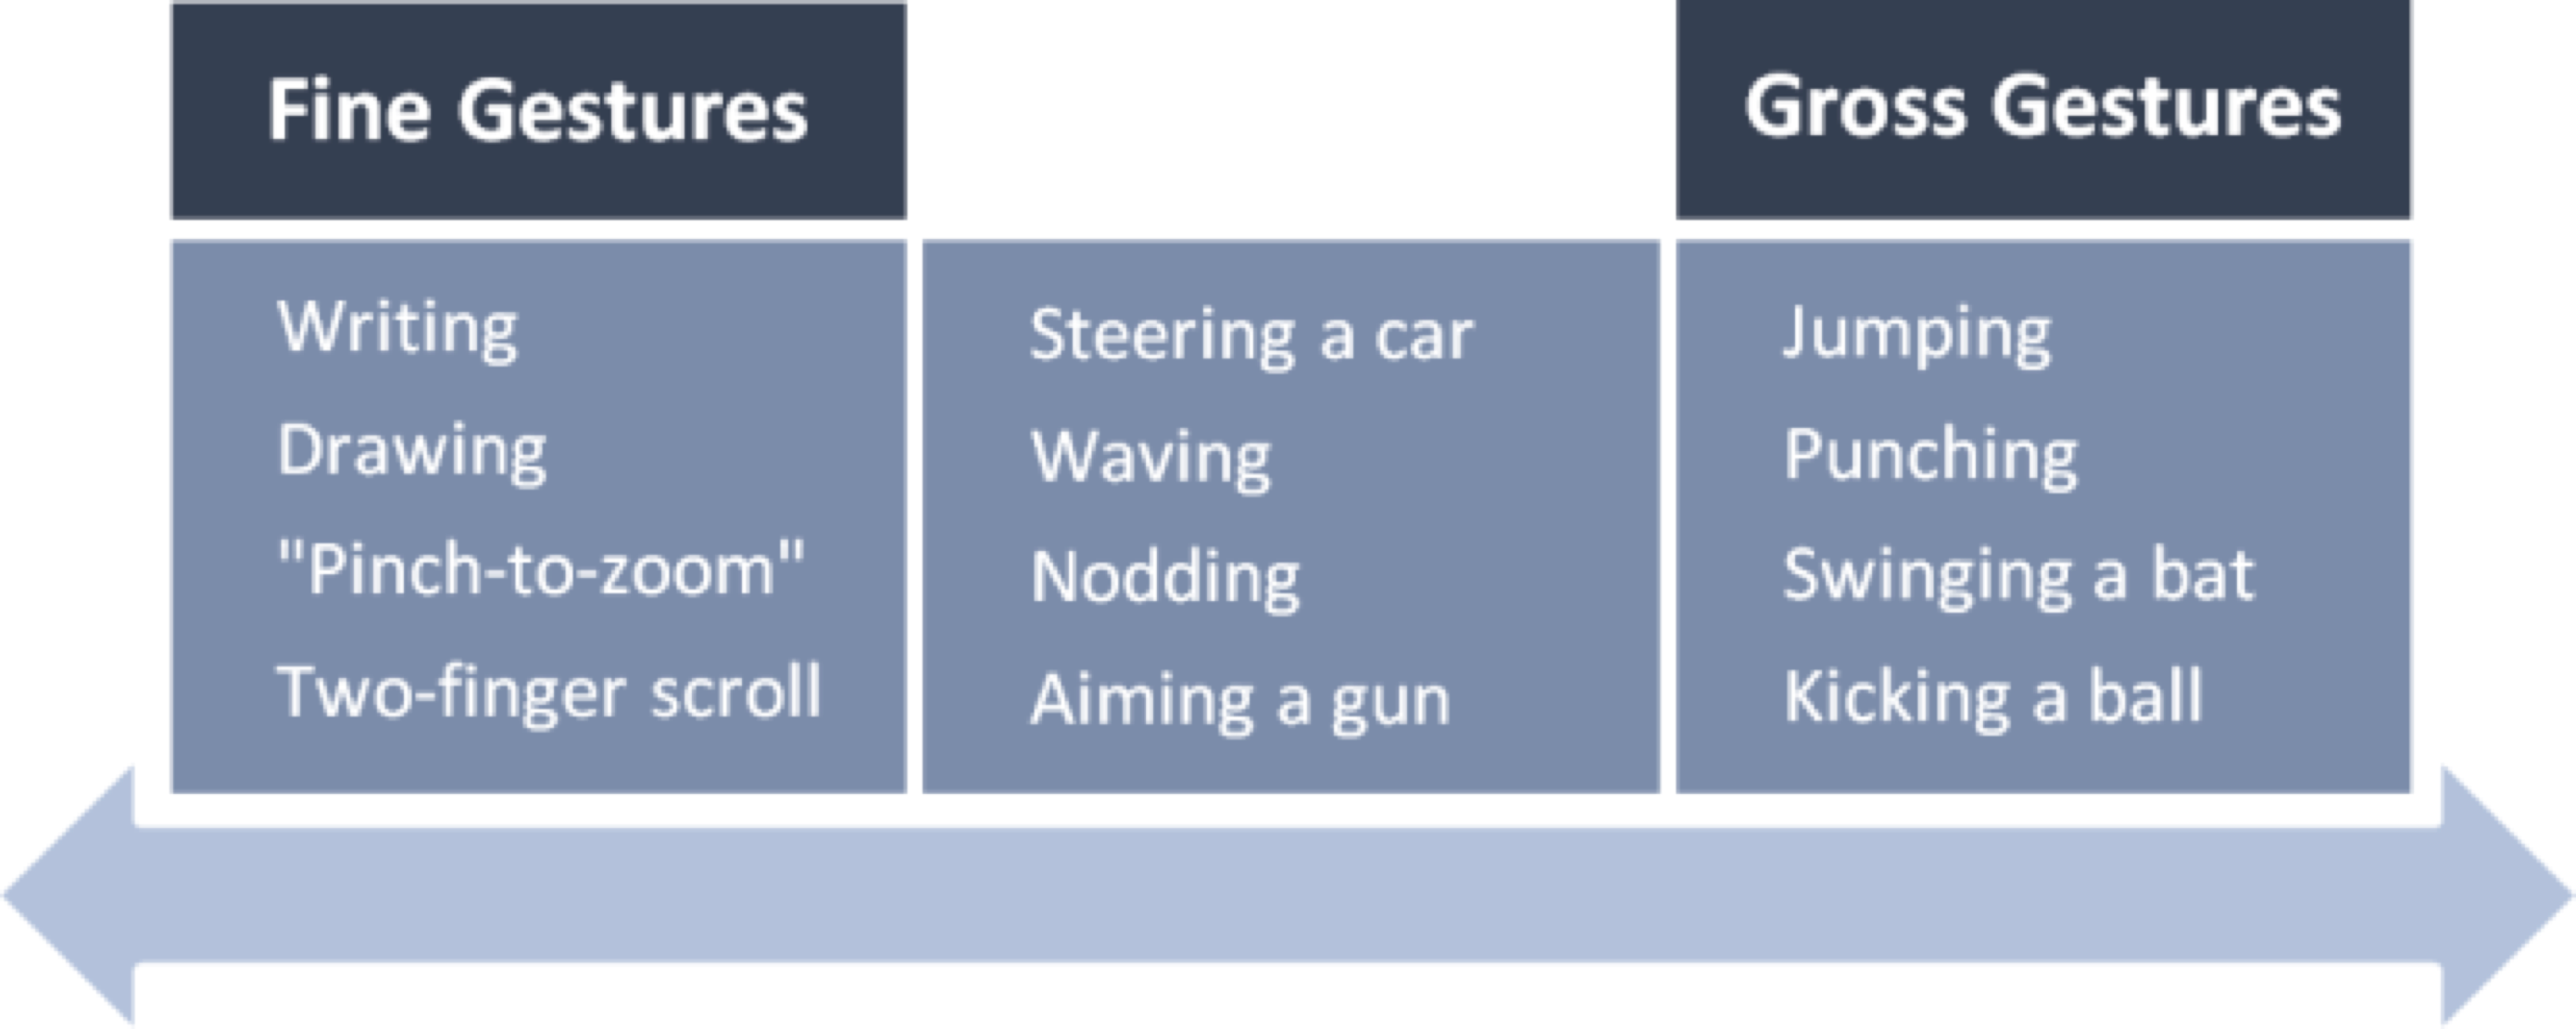
\includegraphics[width=.7\textwidth]{fine-gross-continuum}
\caption{The continuum of \emph{fine} vs. \emph{gross} movements.}
\label{fig:fine-gross-continuum}
\end{SCfigure}

In sum, the scope of this work covers the \hl{design and development of a \emph{software tool for authoring gross mid-air gestures} for interactive computing systems that employ \emph{skeletal tracking perceptual input devices}.}

\begin{table}[ht]
\centering
\renewcommand{\arraystretch}{1.8}
\begin{tabular}{>{\raggedright\arraybackslash}m{.34\textwidth} >{\raggedright\arraybackslash}m{.3\textwidth} >{\raggedright\arraybackslash}m{.27\textwidth}}
\textbf{Aspect} &
\textbf{Coverage} &
\textbf{Excluded Topics} \\
\hline
\textbf{Spatial Qualities of Gestures} &
Mid-Air Gestures &
Surface Gestures \newline Tangibles \newline Pointing Devices \\
\textbf{Gesture Sensing Input Devices} &
Perceptual Input Devices (specifically, Microsoft Kinect) &
Touch Sensors \newline Inertial Sensors \newline Wearables \\
\textbf{Sensor Capabilities} &
Skeletal Tracking &
Hand and Finger Gestures \newline Speech Recognition \newline Image Processing \newline Proxemics \newline Sensor Fusion \\
\textbf{Gestural Bulk\tablefootnote{See Section~\ref{sec:gestural-interaction}.}} &
Gross Movements &
Fine Movements \\
\hline
\end{tabular}
\caption{Summary of the topics covered within and excluded from the scope of the research presented in this thesis.}
\label{tab:scope-summary}
\end{table}

\section{Method}
\label{sec:method}

The method that I adopted to guide the design and development of the gesture authoring tool can be summarized as follows:

\begin{enumerate}
\item \hl{\emph{Prior work}} that may inform the design of a gesture authoring tool for skeletal tracking interfaces is surveyed to \hl{situate the work within the context} of pertinent current research, reveal \hl{design guidelines}, and determine appropriate \hl{strategies for design and evaluation}. Chapter~\ref{chp:background} documents this effort.
\item \hl{\emph{Formative studies}} are conducted with a focus group comprising 10 participants that form a representat sample from the target user populations, using prototypes with varying levels of fidelity. The process and the results of these studies, filtered through the lens of the aforementioned design guidelines, determine the nature and the core features of the gesture authoring tool --- \emph{what} it is going to be. Section~~\ref{sec:formative-studies} describes these studies in detail.
\item The resulting design for the gesture authoring tool is \hl{implemented} as a working application. Various aspects of the implementation are described in Chapter~\ref{chp:hotspotizer}.
\item \hl{\emph{Summative studies}} are conducted to assess if the implementation fulfills the previously stated aims for this work. A user study with 5 participants is conducted to assess the conformance of the artifact with its design rationale. A classroom workshop with 6 participants reveals the tools's potential in supporting rapid prototyping of user interface designs. Section~\ref{sec:summative-studies} describes these studies and their results.
\end{enumerate}
